\begin{figure*}[t!] \centering
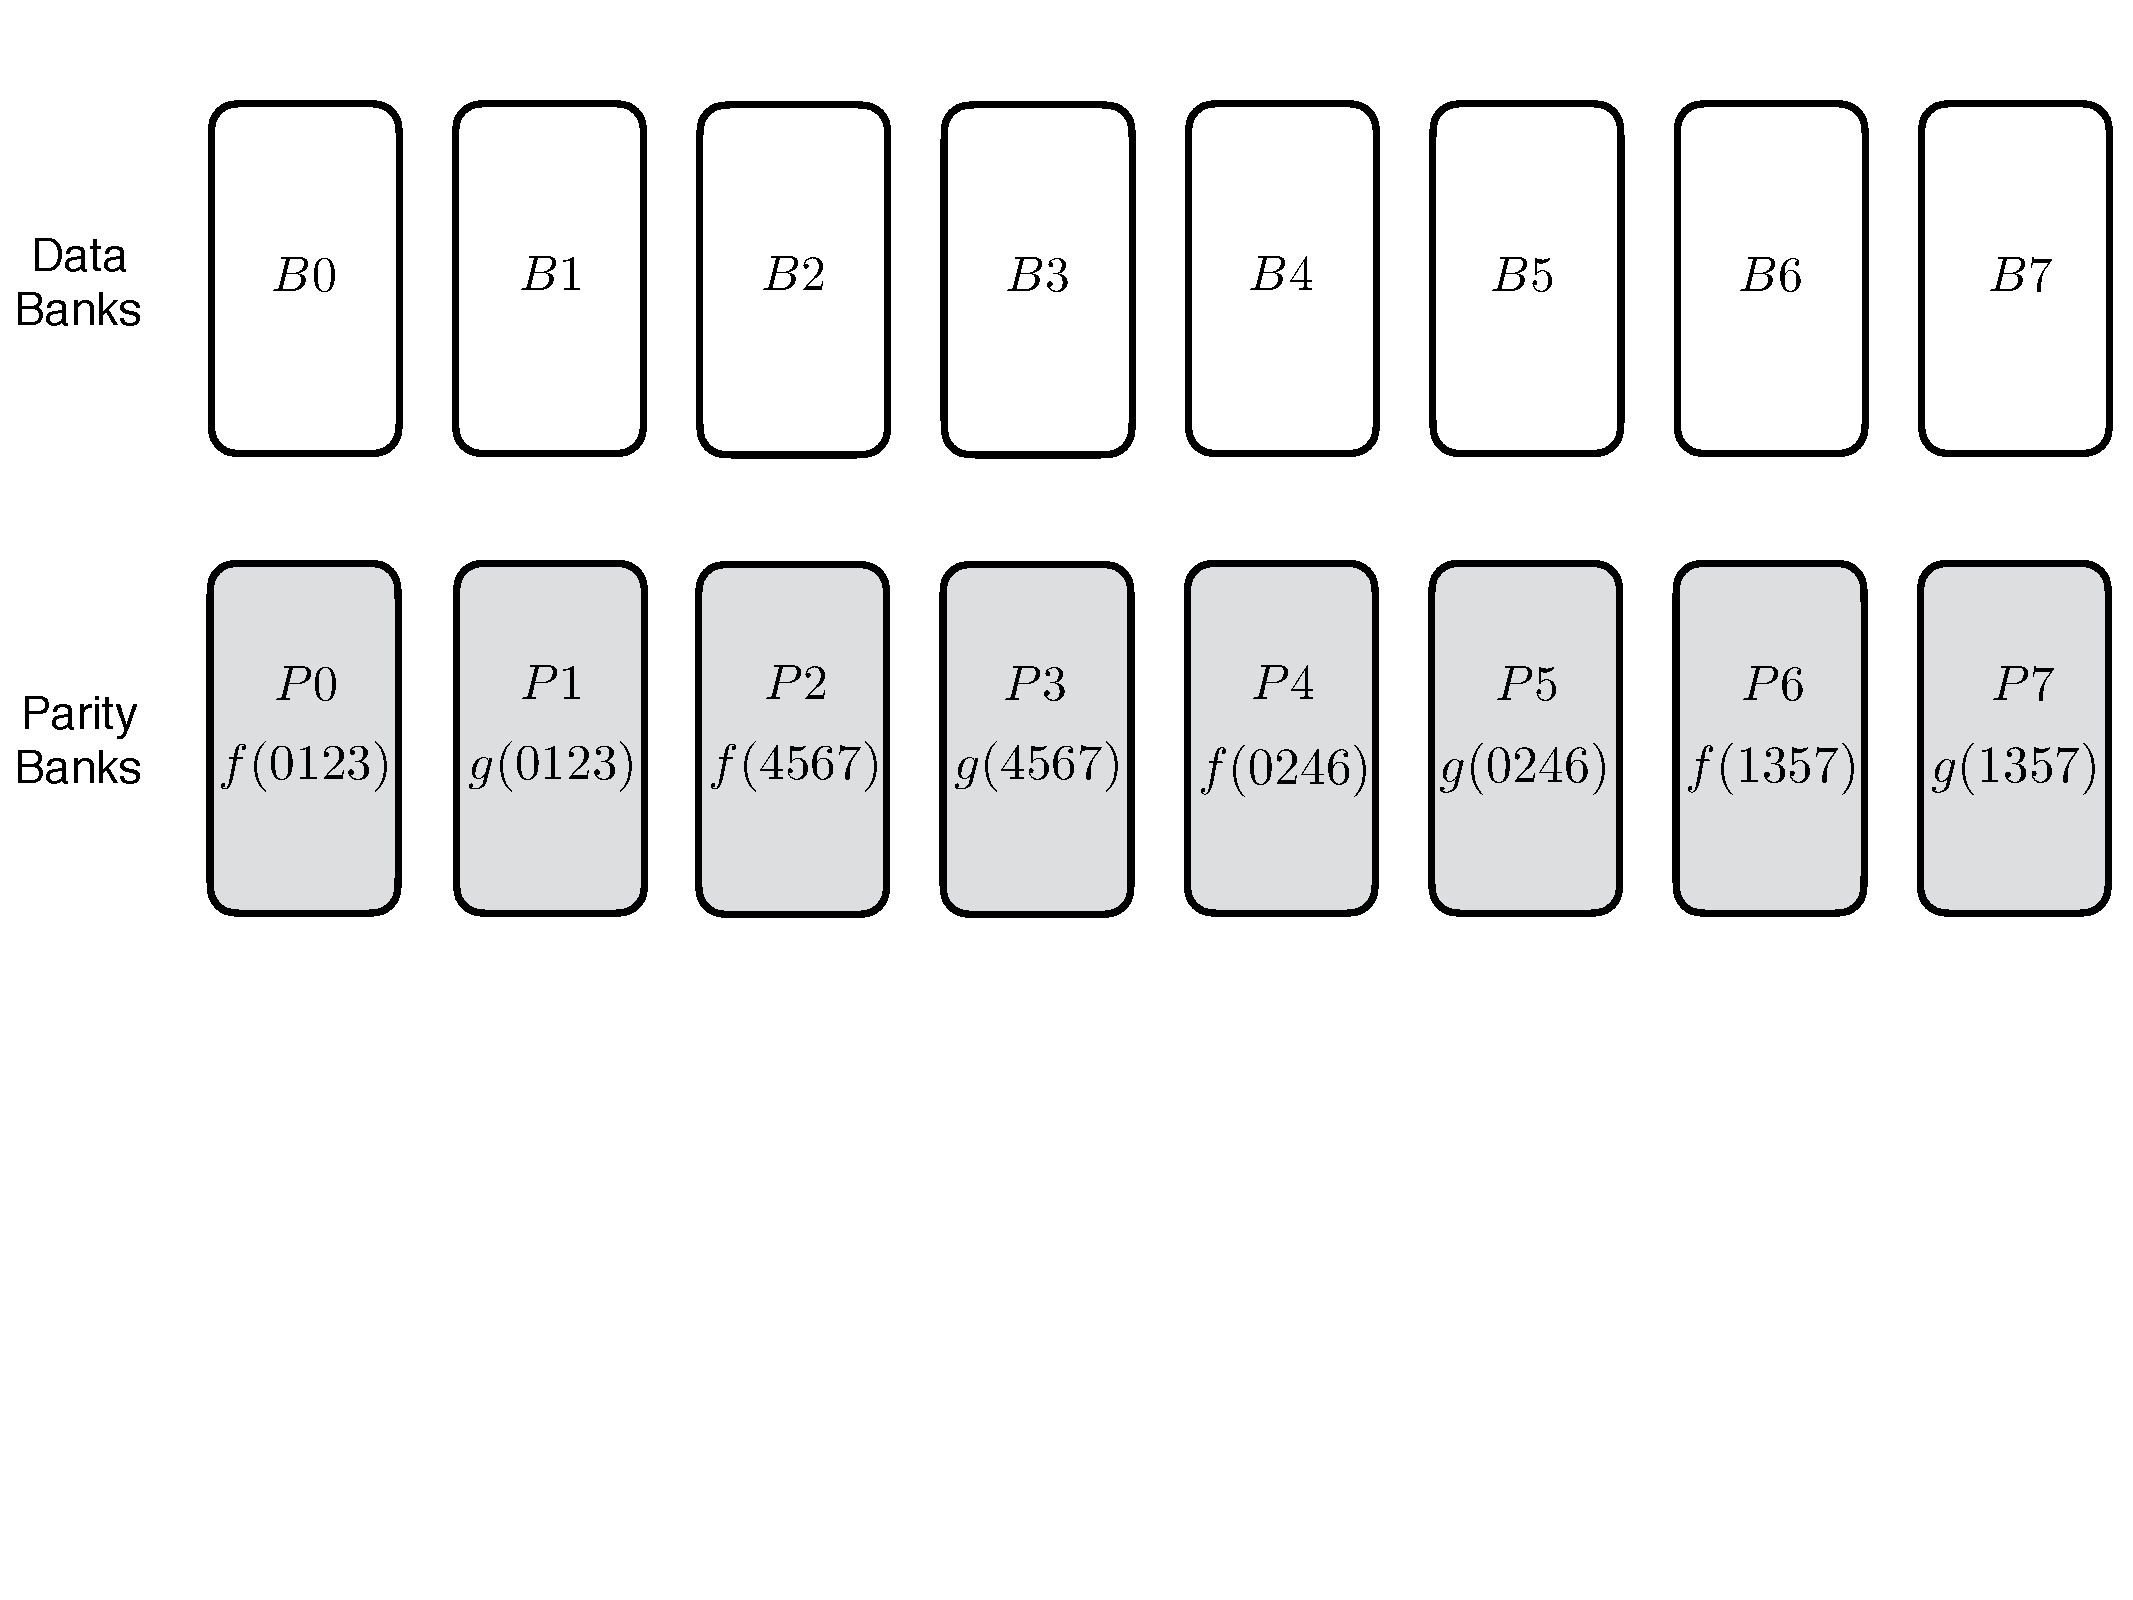
\includegraphics[width=0.7\linewidth]{figures/Code-Design.pdf} 
\caption{Data storage layout for coded memory system}
\label{fig:memsys}
\end{figure*}


\section{CODED MEMORY SYSTEM}
\label{sec:codingArchitecture}

In this paper, we aim to extend the benefits of coding theoretic techniques to dynamic random-access memory systems. In particular, we achieve this by storing the information across single port memory banks in a redundant manner. Traditionally, when multiple requests to a single bank are issued by the cores, a stall occurs as only one address from a single bank can be accessed at a time. As a result, the cores must wait for the first request to the bank be served before their other requests to the bank can be processed. This is where a redundant storage space based on a carefully designed coding scheme comes to the rescue. During a given memory cycle, any data bank that is blocked/busy serving an access can be viewed as a failure as far as other accesses are concerned. Now, other accesses intended for this blocked bank can be served by accessing the content stored in a group of other memory banks. This way, redundant storage space allows concurrent accesses to the same information and alleviates the stalls that are unavoidable in a memory system comprised of non-redundant storage space. 

In this section, we describe our specific memory design in detail. First, we present how to use Reed-Solomon codes to introduce redundancy in the memory storage space. We then discuss the memory controller, the other essential block of our design. Our proposed controller exploits memory bank redundancies to reduce the effect of concurrent read accesses to the stored information. Additionally, the memory controller also maintains consistency and validity of the stored data, which arises due to the presence of write accesses. 




\subsection{Coded Multi-bank Storage Space}
\label{sec:codedBanks}

We rely on a systematic Reed-Solomon (RS) coding scheme as a building block to design the storage space of our proposed memory system. In particular, the storage space consists of $16$ memory banks\footnote{We believe that a $16$ bank design is quite reasonable given that the next generation memory architectures feature many more memory banks than current DRAM architectures.} with $8$ memory banks serving as the data banks and the remaining $8$ banks serving as the parity banks (cf.~Section~\ref{sec:encoding}). As detailed later in this subsection, the parity banks are generated using a systematic $(6,4)$ RS code which is defined over a finite field of size $2^8$, denoted by $GF(2^{8})$.  In any codeword of this systematic $(6,4)$ RS code, it's possible to generate all $4$ associated message symbols given any $4$ symbols of the codeword. 

Before we describe the process of generating the parity blocks, we discuss the reasons behind employing RS codes as opposed to other possible coding schemes. First, RS codes are MDS codes (cf.~Section~\ref{sec:block-codes}), i.e., these codes are optimal in terms of their storage efficiency. 
 Additionally, decades of study has lead to efficient encoding and decoding schemes for RS codes. Crucially, these schemes can be easily \textit{hardcoded} into the memory controller in order to achieve good runtime performance. Finally, RS codes have been proven to be useful in previous work on distributed storage, both in theory and in practice \cite{huang,sathiamoorthy,shanmugam}. In fact, $(14,10)$-RS code is used in production at Facebook in their HDFS-RAID system \cite{sathiamoorthy}. This makes these codes a natural starting point for our dense memory storage architecture.

We now describe the detailed design of the storage space of our proposed memory system. Let the underlying systematic $(6,4)$ RS code map $4$ message symbols $u, v, w, x \in GF(2^{8})$ to a codeword containing $6$ symbols 
$$
\big(u, v, w, x, f(u, v, w, x), g(u, v, w, x)\big) \in GF(2^{8})^6,
$$
where $f, g~:~GF(2^{8})^4 \to GF(2^{8})$ are two linear maps. We arrange the information in $8$ data banks $B0, B1, \ldots, B7$ as shown in Figure~\ref{fig:memsys}. The parity banks $P0, P1,\ldots, P7$ then store the parity symbol which are generated according to the $(6,4)$ RS code described above\footnote{Recall the encoding process and associated notation defined in Section~\ref{sec:encoding}. For example, the functions $f$ and $g$ are applied to the symbols stores in a given row address of $B0, B1, B2,$ and $B3$ to obtain the symbols stored in the same row address of the parity banks $f(0123) \triangleq f(B0,B1,B2,B3)$ and $g(0123) \triangleq g(B0, B1, B2, B3)$, respectively.}. In particular, the first two parity banks $P0$ and $P1$ store the parity symbols that are functions of the information stored in the first four data banks $B0, B1, B2,$ and $B3$. Note that this implies that the symbols stored on the same row address of the six banks $\{B0,\ldots, B3, P0,P1\}$ form codewords of the underlying $(6,4)$ RS code. Similarly, the parity symbols generated from the remaining four data banks $B4, B5, B6,$ and $B7$ are stored in the parity banks $P2$ and $P3$. 

In our design, we ensure that each data bank is part of $2$ codewords of the $(6,4)$ RS code, which are formed by disjoint sets of parity banks. This creates disjoint ways of recovering the information stored in the same data bank. We utilize the parity banks $P4, P5, P6,$ and $P7$ to generate the second codewords associated the data banks. In particular, parity banks $P3$ and $P4$ store the parity symbols generated from the information stored on the even numbered data banks $B0, B2, B4,$ and $B6$. Similarly, the parity banks $P6$ and $P7$ store the parity symbols generated from the odd numbered data banks $B1, B3, B5,$ and $B7$. 

\begin{remark}
\label{rem:degraded}
Note that the redundancy in the storage space helps enable concurrent read accesses by treating the blocked data banks as failures. For example, assume that $B0$ and $B1$ are blocked due to some read accesses. Now, another read access to $B0$ can be realized by using $B2, B3, P0 = f(B0, B1, B2, B3),$ and $P1 = g(B0, B1, B2, B3)$ to recover the symbol in $B0$ required by the access. Similarly, consider a different scenario, where $B0$ is busy serving a read access. Now, another read access for the information stored in $B0$ can be served by reconstructing that information with the help of three data banks $B1, B2, B3,$ and one parity bank $P0 = f(B0, B1, B2, B3)$ or $P1 = g(B0, B1, B2, B3)$.
\end{remark}

%\Ankit{Please somebody rewrite these two lines and then put them in right place...} {\color{blue}The upper part of the bank stores Pseudo Channel 0, and the lower part of the bank stores Pseudo Channel 1. 
%Wherever possible, we try to interleave the banks. This ensures that most large, linear accesses will be spread across multiple banks with reduced contention.}


\subsection{Memory Controller Design}
\label{sec:controller}
The proposed architecture of the memory controller consists of a scheduler which converts memory access requests from the cores into memory access patterns that are mapped to different memory banks. The scheduler has three main components: 1) {\em reorder buffer}, 2) {\em read algorithm}, and 3) {\em write algorithm}. The reorder buffer stores the list of pending or recently served access requests by the memory system. In addition, the reorder buffer also keeps track of the status of the data stored on memory banks as it gets {\em stale} ({\em invalid}) as a result of write requests. The scheduler compares each read and write request to the content of the reorder buffer in order to decide how the request gets served by the read algorithm and the write algorithm, respectively. Next, we describe each of these three main components of the memory controller in detail. 
Table~\ref{fig:rob} shows the behavior of our proposed memory controller architecture on an example request pattern.
%
%\begin{table*}[t!]
% \small
%  \centering
%  \begin{tabular}{c|c|c|c|c|c|c|c|c|c|c|c|c|c|c|c|l}
%    \cline{2-16}
%&    $ROW$ & $Done$ & $R/W$ & $D_{\rm valid}$ & $P_{\rm valid}$ & $DB_{0}$ &  $DB_{1}$ & $DB_{2}$ &$\cdots$ & $DB_7$  & $PB_0$ &  $PB_{1}$ & $PB_{2}$ & $\cdots$ & $PB_7$ \\
%    \cline{2-16}
%t=$1$ &   \texttt{0x2} & 0 & R  & 0 & 0  & 1 & 1 & 0 & 0 & 0 & 0 & 0  & 0 & 0& 0 & {\scriptsize Read $DB_0 - DB_1$}\\
%    \cline{2-16}
%t=$2$ &    \texttt{0x2} & 0 & R & 1 & 1 & 1 & 1 & 1 & 1& 1 & 1& 1 &1 &1&1& {\scriptsize Read $DB_0 - DB_7$}\\
%   \cline{2-16}                          
%t=$3$ &    \texttt{0x2} & 0 & W & 0 & 0 & 0 & 1 & 1 & 1& 1 & 0 & 0 & 0 & 0 & 0 & {\scriptsize Write $DB_0$} \\
%   \cline{2-16}                          
%t=$4$ &    \texttt{0x2} & 0 & W & 1 & 0 & 1 & 1 & 1 & 1& 1 & 0 & 0 & 0 & 0 & 0& \\
%    \cline{2-16}   
%t=$5$ &    \texttt{0x2} & 0 & R & 1 & 0 & 1 & 1 & 1 & 1& 1 & 0 & 0 & 0 & 0 & 0 & {\scriptsize Read $DB_4 - DB_6$}\\
%    \cline{2-16} 
%t=$6$ &    \texttt{0x2} & 1 & R & 1 & 1 & 1 & 1 & 1 & 1& 1 & 1 & 1 & 1 & 1 & 1 &\\
%    \cline{2-16} 
%t=$7$ &    \texttt{0x2} & 1 & R & 1 & 1 & 1 & 1 & 1 & 1& 1 & 1 & 1 & 1 & 1 & 1 &{\scriptsize Read $DB_0 - DB_7$} \\
%    \cline{2-16}                                                     
%  \end{tabular}
%  \caption{Example of a single entry \texttt{0x2} in the reorder buffer across time during a Read-Write-Read request pattern. At t=$1$, there is a read from $DB_0$--$DB_1$, followed by a read at $t=2$ from $DB_0$--$DB_7$ which includes both data and parity banks. A write request to $DB_0$ occurs from $t=3$ to $t=6$, during which $DB_0$ is updated, $D_{\rm valid}$ is set to $1$,  parities $PB_0$--$PB_7$ are updated, $P_{\rm valid}$ is set to $1$, and $Done$ is set to $1$. Since data banks are valid after $t=4$, a read from $DB_{4} $--$DB_6$ is served using only data banks at $t=5$, which sets the $R/W$ bit to $R$. A read from $DB_0 $--$DB_7$ occurs at $t=7$, which does not change the state of the reorder buffer.}
%  \label{fig:rob}
%\end{table*}

\begin{table*}[t!]
 \small
  \centering
  \begin{tabular}{c|c|c|c|c|c|c|c|c|c|c|c|c|c|c|c|l}
    \cline{2-16}
&    $ROW$ & $Done$ & $R/W$ & $D_{\rm valid}$ & $P_{\rm valid}$ & $DB_{0}$ &  $DB_{1}$ & $DB_{2}$ &$\cdots$ & $DB_7$  & $PB_0$ &  $PB_{1}$ & $PB_{2}$ & $\cdots$ & $PB_7$ \\
    \cline{2-16}
t=$1$ &   \texttt{0x2} & 0 & R  & 0 & 0  & 1 & 1 & 0 & 0 & 0 & 0 & 0  & 0 & 0& 0 & {\scriptsize Read $B0 - B1$}\\
    \cline{2-16}
t=$2$ &    \texttt{0x2} & 0 & R & 1 & 1 & 1 & 1 & 1 & 1& 1 & 1& 1 &1 &1&1& {\scriptsize Read $B0 - B7$}\\
   \cline{2-16}                          
t=$3$ &    \texttt{0x2} & 0 & W & 0 & 0 & 0 & 1 & 1 & 1& 1 & 0 & 0 & 0 & 0 & 0 & {\scriptsize Write $B0$} \\
   \cline{2-16}                          
t=$4$ &    \texttt{0x2} & 0 & W & 1 & 0 & 1 & 1 & 1 & 1& 1 & 0 & 0 & 0 & 0 & 0& \\
    \cline{2-16}   
t=$5$ &    \texttt{0x2} & 0 & R & 1 & 0 & 1 & 1 & 1 & 1& 1 & 0 & 0 & 0 & 0 & 0 & {\scriptsize Read $B4 - B6$}\\
    \cline{2-16} 
t=$6$ &    \texttt{0x2} & 1 & R & 1 & 1 & 1 & 1 & 1 & 1& 1 & 1 & 1 & 1 & 1 & 1 &\\
    \cline{2-16} 
t=$7$ &    \texttt{0x2} & 1 & R & 1 & 1 & 1 & 1 & 1 & 1& 1 & 1 & 1 & 1 & 1 & 1 &{\scriptsize Read $B0 - B7$} \\
    \cline{2-16}                                                     
  \end{tabular}
  \caption{Example of a single entry \texttt{0x2} in the reorder buffer across time during a Read-Write-Read request pattern. At t=$1$, there is a read from $B0$--$B1$, followed by a read at $t=2$ from $B0$--$B7$ which includes both data and parity banks. A write request to $B0$ occurs from $t=3$ to $t=6$, during which $DB_0$ is updated, $D_{\rm valid}$ is set to $1$, bits for parities banks, i.e., $PB_0$--$PB_7$, are updated, $P_{\rm valid}$ is set to $1$, and $Done$ is set to $1$. Since data banks are valid after $t=4$, a read from $B{4} $--$B6$ is served using only data banks at $t=5$, which sets the $R/W$ bit to $R$. A read from $B0 $--$B7$ occurs at $t=7$, which does not change the state of the reorder buffer. \Matt{Why does writing to B0 set all PB bits to 0? not all parity banks are a function of B0.}}
  \label{fig:rob}
\end{table*}

\subsubsection{Reorder buffer}
\label{sec:reorder}

As mentioned earlier, all access requests need to go through the reorder buffer. The reorder buffer stores the data downloaded from the memory banks in order to serve read access requests from the cores. Similarly, the reorder buffer also stores the new data that arrives with write requests and need to be written on the coded memory banks (after generation of consistent parity data). In addition to storing the actual data, the reorder buffer maintains metadata to keep track of the rows of the memory banks that are present in the reorder buffer and the validity of these rows across data banks and parity banks. Each write request invalidates the content of (some of) the data banks. The data on these banks (and on the corresponding parity banks which depend on them) then needs to be updated. The metadata of the reorder buffer is used to ensure this consistency across the data and parity banks when the memory controller maps a write request to be written on the memory banks. The reorder buffer size is a key design parameter which trades off faster access speeds for increased overhead, as shown in Section~\ref{sec:experiments}.


For each row address in the memory banks, the reorder buffer stores {\em at most $1$} entry along with the following $20$ bits of metadata (cf.~Table~\ref{fig:rob}). 
\begin{itemize}
\item {$Done$:~}This bit indicates if this particular row address had a write request associated with it in the past that has not yet been written to the memory banks. If $Done$ bit is set to $1$, this implies that this row address was affected by the write requests and the content on the memory banks need to be updated when this row is removed from the metadata of the reorder buffer.
\item {$R/W$:~} This bit denotes the nature of the most recent access request for the row address associated with the entry in reorder buffer. $R$ and $W$ refers to the read request and the write request, respectively.
\item {$D_{\rm valid}$:~}This bit indicates if the reorder buffer stores the valid data for the corresponding row address in each of the {\em data} banks. $D_{\rm valid}$ bit is set to $1$ when the reorder buffer has the valid copies of the content for all the data banks.
\item {$P_{\rm valid}$:~}This bit indicates if the reorder buffer stores the valid data for the corresponding row address in each of the {\em parity} banks. $P_{\rm valid}$ bit is set to $1$ when the reorder buffer stores the valid copies of the data for all the parity banks.
\item {$DB_0, \ldots, DB_7$:~}Similar to the $D_{\rm valid}$ bit, for $0 \leq i \leq 7$, $DB_{i}$ bit is set to $1$ to denote that the reorder buffer stores the valid data for the associated row address in the $i$-th data bank $Bi$.
\item {$PB_0, \ldots, PB_7$:~}Similar to the $P_{\rm valid}$ bit, for $0 \leq i \leq 7$, $PB_{i}$ bit is set to $1$ to indicate that the reorder buffer stores the valid version of the content for the associated row address in the $i$-th parity bank $Pi$.
\end{itemize}
Note that $D_{\rm valid}$ and $P_{\rm valid}$ are logical $AND$s  of $DB_{0}-DB_{7}$ and $PB_{0}-PB_{7}$, respectively. 
\begin{remark}
Even though the data stored in a particular row in the memory banks might be invalid, the reorder buffer may store its valid version which would lead to the $D_{\rm valid}$ and/or $P_{\rm valid}$ bits to be set. It's the responsibility of the write algorithm to transfer this valid data from the reorder buffer to the memory banks when the corresponding row is evicted from the reorder buffer.
\end{remark}

\begin{remark}
\label{rem:priority}
Here, we note that the reorder buffer can also be utilized to incorporate different priority levels among access requests, if the memory systems is required to support multiple access types with different priority levels.
\end{remark}


\subsubsection{Read algorithm}
\label{sec:read}

For a given state of the reorder buffer and the set of pending read requests from the cores, the main purpose of the read algorithm is to maximize the number of read requests that can be served in a given memory cycle. This is accomplished by utilizing the redundant parity banks in an efficient manner without increasing the algorithm's overall complexity. Note that in our coded memory design (cf.~Section~\ref{sec:codedBanks}), a parity bank is useful during data access only if some of the corresponding data banks are also accessed. In particular, assuming that all the relevant parity banks are valid, there are two possible ways of serving a read request by employing the parity banks: 1) content of $2$ data banks and $2$ parity banks is utilized; and  2) content of $3$ data banks and $1$ parity bank is utilized (cf.~Remark~\ref{rem:degraded}). In every cycle, the scheduler picks pending read requests {\em in order} and tries to serve them according to the read algorithm described in Figure~\ref{fig:read}. In addition to this, whenever all but $1$ data bank is present in the buffer, that data bank is automatically read from memory and the algorithm proceeds with $D_{\rm valid}$ set to $1$. \Matt{Read algorithm questions:
1) Where is the R/W bit set to read?
2) Regarding the $D_{valid} = true$ condition, Why does $D_{valid}$ need to be true to serve a request? Say I want to read from B0, and the DB0 bit is set. There is enough information in the Reorder buffer to serve the request. Why should I care if $D_{valid}$ is set?}
%-------------------------------------------------------------------------
\begin{figure}[h!] \centering
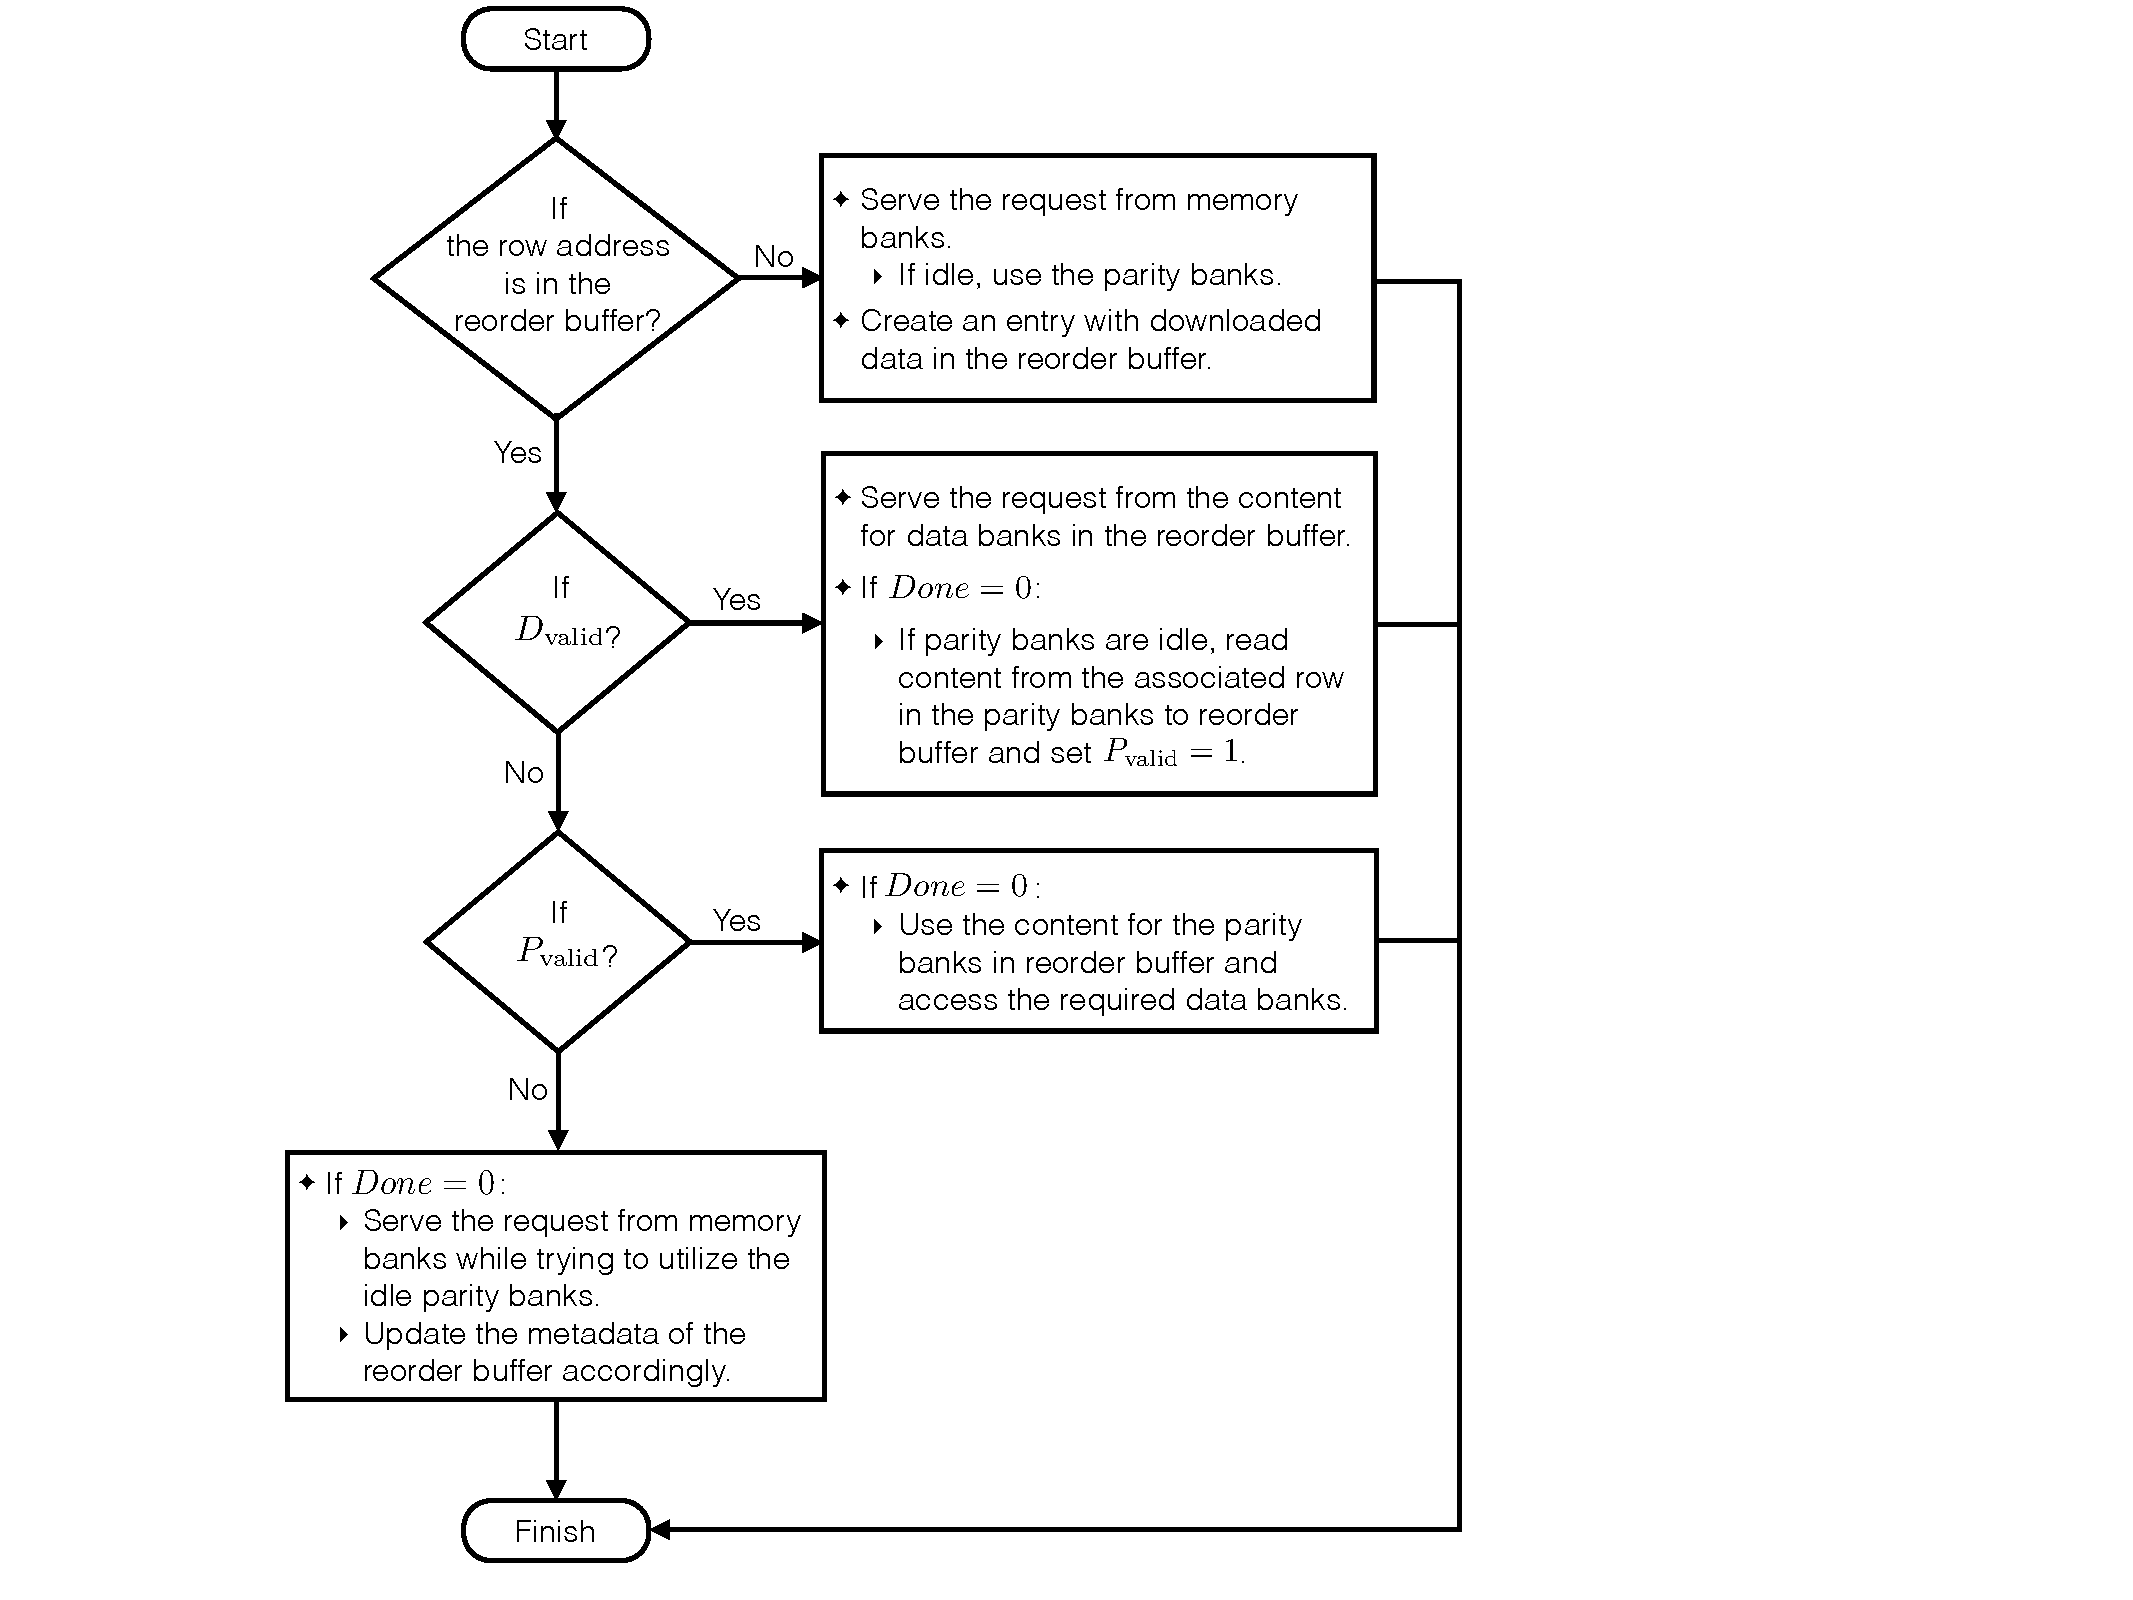
\includegraphics[width=0.85\linewidth]{figures/Read-algo-new.pdf} 
\caption{Description of the read algorithm.}

\label{fig:read}
\end{figure}
%-------------------------------------------------------------------------

\subsubsection{Write algorithm}
\label{sec:write}
Note that each write request is accompanied by the content that needs to be updated in (some of) the data banks. However, in order to have consistency across all the memory banks, every update in the data banks should be reflected in the associated parity banks as well. The write algorithm ensures that the reorder buffer stores consistent and valid data for each row address available in the buffer. The write algorithm achieves this task by following the procedure described in Figure~\ref{fig:write}. In particular, the write algorithm picks the pending write access requests from the core in order. The algorithm then determines if the associated row address is present in the reorder buffer. If it is not present, it makes an entry for the row in the reorder buffer. \Matt{Why set every parity bank bit to 0 when performing a write? Suppose you write to DB0. That shouldn't effect parity banks which are not functions of DB0}

\begin{figure}[h!] \centering
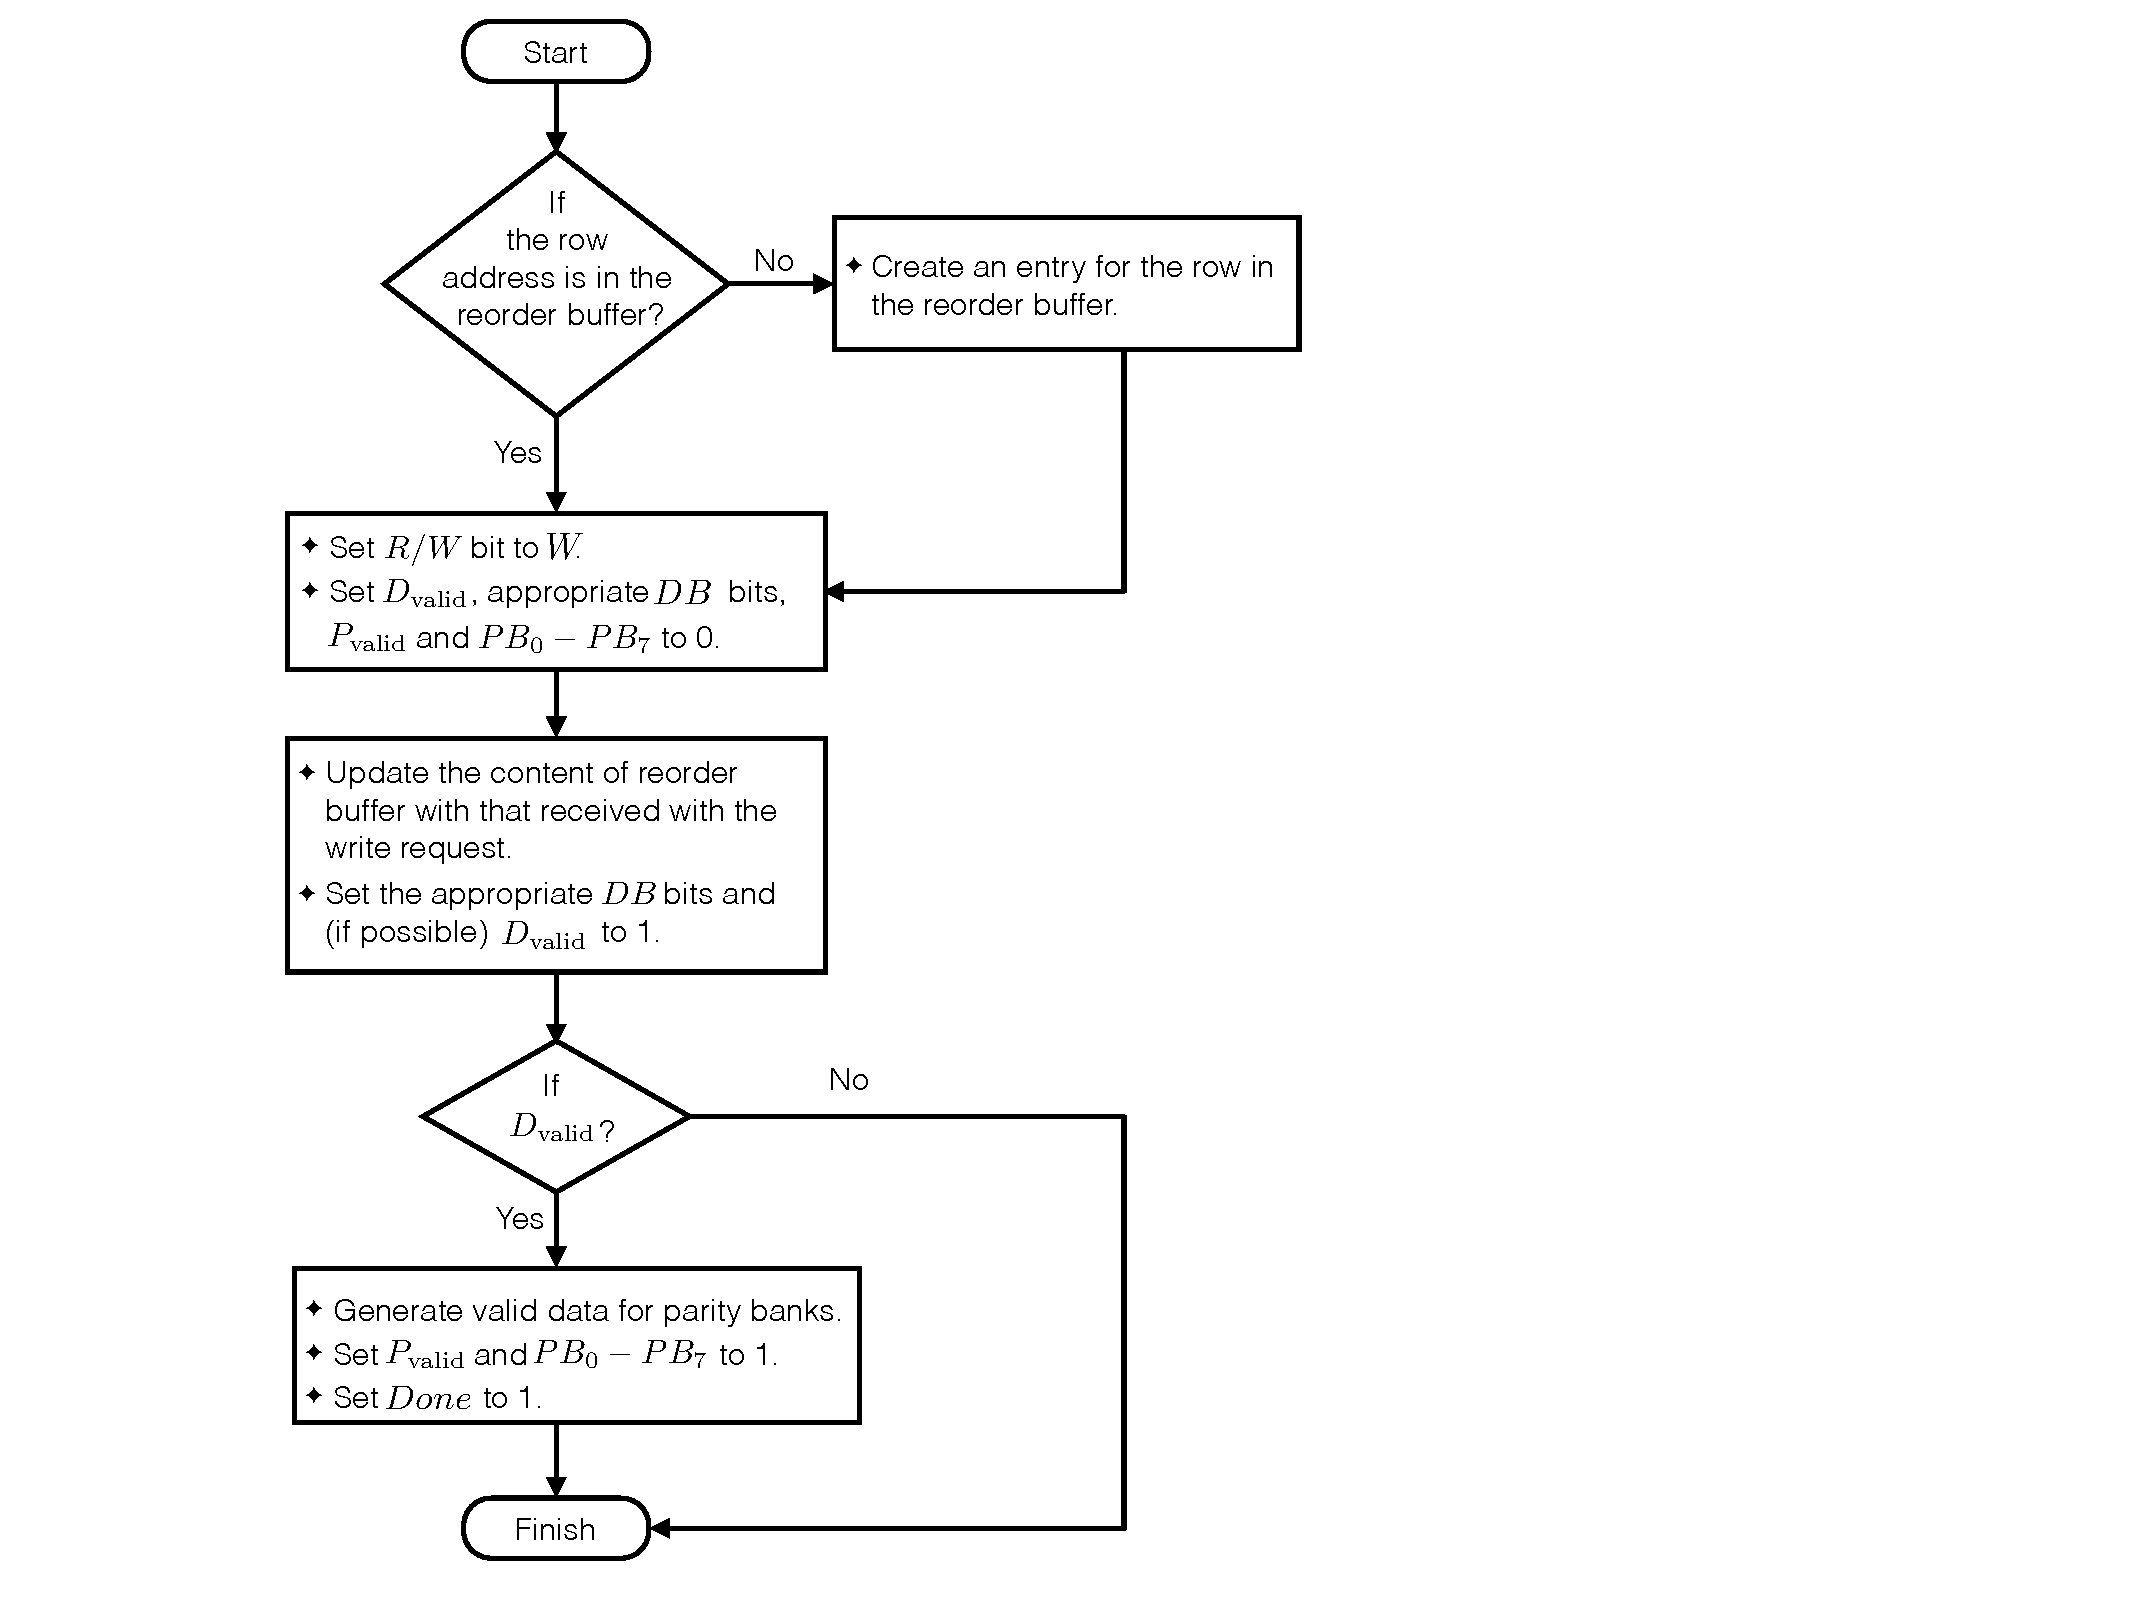
\includegraphics[width=0.80\linewidth]{figures/Write-algo-new.pdf} 
\caption{Description of the write algorithm.}
\label{fig:write}
\end{figure}


Once the reorder buffer has the entry for the row address, the write algorithm ensures that the buffer stores the valid content for the row address. This involves 1) copying the content received with the write request to update the content already available in the buffer from the data banks; 2) regenerating the updated content for the parity banks; and 3) updating the metadata of reorder buffer by modifying the entry corresponding to the underlying row address. Once the reorder buffer has valid and consistent data for a given row address, $Done$ is set to $1$. 

Table~\ref{fig:rob} illustrates these steps for an example write request. At $t = 3$, the write algorithm starts processing a write request for data bank $B0$ by setting the $R/W$ bit with the associated address to $W$. It also sets the $D_{\rm valid}$, $DB_{0}$, $P_{\rm valid}$ and $PB_{0}-PB_{7}$ to zero. In the subsequent steps, the write algorithm updates the content for data bank $B0$ in the buffer by replacing it with the content received with the write request. It then updates $DB_0$ and $D_{\rm valid}$ by setting those to $1$. If $D_{\rm valid}$ is $0$, the reorder buffer entry remains in the buffer until all data banks are updated. Once $D_{\rm valid}$ is indeed $1$, then the write algorithm generates the new content for the parity banks and sets $P_{\rm valid}$ and $PB_0 -PB_7$ to $1$. At this point, it also sets $Done$ to $1$.

Once the $Done$ bit is set to $1$, the write algorithm schedules the updated row to be written to the memory banks. Once the write is successfully performed on the memory banks, the entry in the reorder buffer is updated by setting $R/W$ bit to $R$ and $Done$ bit to $0$. Here, we note that the $R/W$ bit can get modified by a subsequent read request (as illustrated in Table~\ref{fig:rob}). However, the $Done = 1$ bit reminds the scheduler that the memory banks have not yet been updated.


%{\color{red}The write request is now considered successfully processed as far as the writing algorithm is considered. Note that the content stored on the memory banks has not been updated up to this point. This task of performing the updates on memory banks is handled by the writeback algorithm (cf. Section~\ref{sec:writeback}, which is invoked every time an entry is evicted from the reorder buffer.}

\subsubsection{Writeback algorithm}
\label{sec:writeback}
The scheduler uses the limited size reorder buffer to fetch data from the bank rows and to perform read, write and code operations. In the process, the scheduler ensures that every time the reorder buffer reaches near its capacity, it clears up entries based on the following set of rules: Rule 1 is to pop out the oldest entry in the reorder buffer. Rule 2 is to ensure that the evicted row from the reorder buffer matches the data in the memory bank. This is ensured by using the $Done$ bit in the reorder buffer. If a write instruction modifies a data bank entry, the scheduler reconstructs the code and makes $Done = 1$. 